\documentclass[10pt]{elegantbook}

\title{Machine Learning Notes}
\subtitle{All in the data.}

\author{occupymars}
\date{June. 23, 2025}
\version{0.1}

\cover{iron_man.jpg}

% all the packages included
\usepackage{cprotect}
\usepackage{fontawesome}
\usepackage[linesnumbered, ruled]{algorithm2e}
\RestyleAlgo{algoruled}

% set some fonts
\setmonofont{Ubuntu Mono}

% my own commands
% \newcommand{\mydefination}[1]{\textit{\textcolor[RGB]{0,174,247}{#1}}}
\newcommand{\mydefination}[1]{\textbf{\textit{\textcolor{structurecolor}{#1}}}}

\begin{document}

\maketitle

\frontmatter
\tableofcontents

\mainmatter

\chapter{Survey Papers}

\begin{introduction}
    \item Gaussian Process (2025)
\end{introduction}

\section{Gaussian processes for dynamics learning in model predictive control (2025)}

\subsection{Overview of static Gaussian process regression}

GPR was introduce in the statistics community by \textit{Curve Fitting and Optimal Design for Prediction}, and gained
attention after \textit{Bayesian Learning for Neural Networks} proved that they can be regarded as neural networks of infinite
width.

Given two input data $Z = \{ z_1, \cdots, z_N \}, Z^* = \{ z^*_1, \cdots, z^*_N \}$, using the GP prior, we get:
\[
\begin{bmatrix}
    g_Z \\ g_{Z^*}
\end{bmatrix} \sim \mathcal N 
\left (
\begin{bmatrix}
    0 \\ 0
\end{bmatrix},
\begin{bmatrix}
    \mathscr{K}_{Z, Z} & \mathscr{K}_{Z, Z^*} \\
    \mathscr{K}_{Z^*, Z} & \mathscr{K}_{Z^*, Z^*}
\end{bmatrix}    
\right )
\]

Now given observation for $Z$ as $Y = [y_1, \cdots, y_N]$, the posterior can be written as:
\[
p(g_Z, g_{Z^*} \mid Y) = \frac{p(Y \mid g_Z)p(g_Z, g_{Z^*})}{p(Y)}
\]

The kernel is often taken as Gaussian one:
\[
\mathscr{K}_{Z, Z^*} = \lambda \exp \left \{ -\frac{\| Z - Z^* \|^2}{2 \eta} \right \}
\]

If we are using the measurement model $y_i = g(z_i) + w_i$ and assume noise term is independent from prior $g$:
\[
Y \mid g_Z \sim \mathcal N (g_Z, \sigma_w^2 I_N)
\]
so the posterior is also Gaussian, we can get the posterior of interest:
\[
p(g_{Z^*} \mid Y) = \int_{\mathcal Z} \frac{p(Y \mid g_Z)p(g_Z, g_{Z^*})}{p(Y)} dg_Z
\]
then compute the first and second order moments, we get $g_{Z^*} \mid Y \sim \mathcal N (\mu(Z^*), \Sigma(Z^*))$:
\begin{equation} \label{eq:gp_mean_cov}
\left \{
\begin{array}{lll}
    \mu(Z^*) &=& \mathscr{K}_{Z^*, Z} (\mathscr{K}_{Z, Z} + \sigma_w^2 I_N)^{-1} Y \\
    \Sigma(Z^*) &=& \mathscr{K}_{Z^*, Z^*} - \mathscr{K}_{Z^*, Z} (\mathscr{K}_{Z, Z} + \sigma_w^2 I_N)^{-1} \mathscr{K}_{Z, Z^*}
\end{array}    
\right .
\end{equation}

\begin{remark}
    1, Alternative paradigms for uncertainty quantification, from RKHS to multi-arm bandits, frequency methods...
\end{remark}

The hyperparameters are estimated from a subset of data $(Z_h, Y_h)$ by optimizing the marginal likelihood:
\begin{equation} \label{eq:hyper_opt}
\text{argmax}_{\xi} ~ p(Y_h \mid \xi) = \text{argmax}_{\xi} ~ \int_{\mathbb R^N} p(Y_h \mid g_{Z_h}, \xi)p(g_{Z_h} \mid \xi)dg_{Z_h}
\end{equation}
if the measurement is i.i.d., then $Y_h \mid \xi \sim \mathcal N(0, \mathscr{K}_{Z_h, Z_h} + \sigma_w^2)$, so the above optimization
problem can be written as a negative-log-likelihood minimization problem:
\begin{equation} \label{eq:hyper_nll_opt}
\text{argmax}_{\xi} ~ Y_h^{\top}(\mathscr{K}_{Z_h, Z_h} + \sigma_w^2)^{-1}Y_h + \log \det(\mathscr{K}_{Z_h, Z_h} + \sigma_w^2)
\end{equation}
we can use a gradient based method to optimize this one, however this cost is not convex, so its result maybe not global minimum and 
thus unreliable. An alternative way is \mydefination{Markov Chain Monte Carlo} approaches, perform numerical integration on \ref{eq:hyper_opt}.

\subsection{Gaussian processes for dynamical systems}
A first option to describe a dynamical system is the Nonlinear, Auto-Regressive with eXogenous input (\mydefination{NARX}) model:
\[
y_i = g_{NARX}(y_{i-1}, \cdots, y_{\tau_y}, u_{i-1}, \cdots, u_{\tau_u}) + w_i
\]

We can write it as the state-space model:
\begin{equation}
    \left \{ 
    \begin{array}{rll}
        x_{i+1} &=& f(x_i, u_i) + v_i \\
        y_i &=& g(x_i) + w_i
    \end{array}    
    \right .    
\end{equation}
where $f$ and $g$ denotes transition and emission maps, typically $g$ is known (even if it is not, we can augment it into 
transition maps). There are two challenges, learning two maps and state inference (from $y$ get $x$), that is tackled by two
different approaches in academic:
\begin{itemize}
    \item Optimizing latent state variables: treate the state variables as optimization variables, jointly optimize it with 
model parameters to get maximum likelihood.
    \item Alternating function learning and state inference: this method try to extend Bayesian techniques such as 
\mydefination{Extended Kalman Filter}, \mydefination{Unscented Kalman Filter}, Assumed Density Filter, and Particle Filter 
to non-parametric models, the approximation in these 
studys are Taylor expansions, exact moment matching and particle representations. But when the state measurement
are not available, we have to iteratively alternate between inferring the posterior and updating $ \xi $ to maximize the 
marginal likelihood, using algorithm like \mydefination{Expectation Maximization}. The approximation to decrease the computational
complexity are truncated orthogonal basis functions expansions (see [132, 133, 134]) and variational inference.
\end{itemize}

\subsection{Porblem formulation}
The discrete model dynamic:
\begin{equation} \label{eq:gp_dynamic_model}
    x_{i+1} = g_{nom}(x_i, u_i) + B_d g(x_i, u_i) + v_i
\end{equation}
where $g_{nom}: \mathbb R^{n_x \times n_u} \rightarrow \mathbb R^{n_x}, g: \mathbb R^{n_x \times n_u} \rightarrow \mathbb R^{n_d}$, 
if we do not have nominal model, then $B_d = I_{n_x}$.

And we use $z_i = [x_i^{\top} \quad u_i^{\top}]^{\top}$, we will train $n_d$ GPs for each dimension separately.

The optimal control problem is then:
\begin{align}
    \text{minimize}_{\{\pi_i\}} \quad & \mathbb{E} \left[ \bar{\mathcal{L}}_{\bar T}(x_{\bar T}) + \sum_{i=0}^{\bar T-1} \mathcal{\bar L_i}(x_i, u_i) \right] \\
    \text{subject to} \quad & x_{i+1} = g_{\text{nom}}(x_i, u_i) + B_d g(x_i, u_i) + v_i \\
    & u_i = \pi_i(x_i) \\
    & \mathbb{P}(h_j(x_i, u_i) \leq 0, \forall i \geq 0) \geq p_j \quad \forall j=1,\ldots,n_h \\
    & x_0 = \bar{x}_0
\end{align}

This problem is hard to solve, so we transform it to a MPC problem at time step $k$:
\begin{align}
    \text{minimize}_{\{\pi_i | k\}} \quad & \mathbb{E} \left[ \mathcal{L}_{T}(x_{T|k}) + \sum_{i=0}^{T-1} \mathcal{L_i}(x_{i|k}, u_{i|k}) \right] \\
    \text{subject to} \quad & x_{i+1|k} = g_{\text{nom}}(x_{i|k}, u_{i|k}) + B_d g(x_{i|k}, u_{i|k}) + v_{i|k} \\
    & u_{i|k} = \pi_{i|k}(x_{i|k}) \\
    & \mathbb{P}(h_j(x_{i|k}, u_{i|k}) \leq 0, \forall i \geq 0) \geq p_j \quad \forall j=1,\ldots,n_h \\
    & x_{0|k} = x_k
\end{align}

\subsection{Scalable methods for GPR}
More detailed survey please refer to \textit{When Gaussian Process Meets Big Data: A Review of Scalable GPs}.

\begin{table}[ht]
\centering
\caption{Computational Complexity of Gaussian Process Methods.}
\begin{tabular}{lccccccc}
\toprule
& GP Full & Subset of Data & Expert-based & FTC & SSGP & SKI & SVGP \\
\midrule
Training  & $\mathcal O(N^3)$ & $\mathcal O(M^3)$ & $\mathcal O(NM_e^2)$ & $\mathcal O(NM^2)$ & $\mathcal O(Np^2)$ & $\mathcal O(N + M \log M)$ & $\mathcal O(M^3)$ \\
Inference & $\mathcal O(N^2)$ & $\mathcal O(M^2)$ & $\mathcal O(M_e^2)$  & $\mathcal O(M^2)$  & $\mathcal O(p^2)$  & $\mathcal O(M \log M)$     & $\mathcal O(M^2)$ \\
\bottomrule
\end{tabular}
\end{table}

\mydefination{1. Subset of Data}, sample data using some criterion (refer to \textit{Gaussian Process Models: PAC-Bayesian 
Generalisation Error Bounds and Sparse Approximations}, chapter 4) and clustering. This will overestimate uncertainty, but 
new study leveraging graphons complementss rigorous bounds for it. 

We can also use multiple models for different regions for non-Stationarity or scalability. One of them is called \mydefination{Mixture-of-Experts}
(MoE), given $N_{exp}$ GPs, denoting with $\{ s_k(\cdot) \}_{k=1}^{N_{exp}}$ a set of gating functions, the overall likelihood is
\[
p_{MoE}(y \mid g_z^1, \cdots, g_z^{N_{exp}}) = \sum_{k=1}^{N_{exp}} s_k(g_z^k)p_k(y \mid g_z^k)
\]
to scale well, we need to use infinite MoE or one of the approximation methods. We can also pre-allocate experts but this will
lose connection between experts. See [166], [167] for online updates. And there is another method called "bagging".

Instead of resorting to a linear combination of GPs, we can use \mydefination{Product-of-Experts} (PoE), where
\[
p_{PoE}(y \mid g_z^1, \cdots, g_z^{N_{exp}}) \propto \prod_{k=1}^{N_{exp}} p_k(y \mid g_z^k)
\]
this will make weak expert plays which is not good, so we can use weighted product and Bayesian Committee Machine, combined
we have [174]. MoE and PoE combine in \textit{Deep Structured Mixtures of Gaussian Processes}. Analysis of theory 
in \textit{An asymptotic analysis of distributed nonparametric methods}.

\mydefination{2. Inducing Variables}, given inducing points (pseudo-inputs) $\bar Z$ and $g_{\bar Z} \sim \mathcal N(0, \mathscr{K}_{\bar Z, \bar Z})$, 
$g_Z$ and $g_{Z^*}$ are conditionally independent, they can only communicate through $g_{\bar Z}$. There are two main groups,
one is approximate prior $p(g_Z, g_{Z^*})$ and do exact inference (reviewed in \textit{A Unifying View of Sparse Approximate Gaussian Process Regression}),
one is from original prior and approximate $p(g_{Z^*} \mid Y)$ (reviewed in \textit{A unifying framework for Gaussian process pseudo-point approximations using power expectation propagation}),
they are compared in \textit{Understanding Probabilistic Sparse Gaussian Process Approximations}.

First we talk about method approximating prior, with:
\begin{equation}
    \begin{array}{rll}
        p(g_{Z},g_{Z^{*}}) &=& \int p(g_{Z},g_{Z^{*}}|g_{\bar Z})p(g_{\bar Z})d g_{\bar Z} \\ 
        &\approx&\int q(g_{Z}|g_{\bar Z})q(g_{Z^{*}}|g_{\bar Z})p(g_{\bar Z})d g_{\bar Z} \\
        &=& q(g_{Z},g_{Z^{*}})
    \end{array}
\end{equation}
the choice of $q(g_{Z}|g_{\bar Z}) = \mathcal N(\mathscr{K}_{Z, \bar Z}\mathscr{K}_{\bar Z, \bar Z}^{-1}g_{\bar Z}, \tilde Q_{Z, Z})$ 
and $q(g_{Z^{*}}|g_{\bar Z}) = \mathcal N(\mathscr{K}_{Z^*, \bar Z}\mathscr{K}_{\bar Z, \bar Z}^{-1}g_{\bar Z}, \tilde Q_{Z^*, Z^*})$ 
will differ between different methods below. The conditional distribution is actully $q(g_{Z}|g_{\bar Z}) = \mathcal N(\mathscr{K}_{Z,
 \bar Z}\mathscr{K}_{\bar Z, \bar Z}^{-1}g_{\bar Z}, \mathscr{K}_{Z, Z} - \mathscr{K}_{Z, \bar Z}
 \mathscr{K}_{\bar Z, \bar Z}^{-1}\mathscr{K}_{\bar Z, Z}$), 
refer to \href{https://statproofbook.github.io/P/mvn-cond.html}{proof}, $\tilde Q$ is a low rank matrix.
\begin{itemize}
    \item \mydefination{Subset of Regressors} (SoR), $\mathscr{K}_{Z, Z} \approx \mathscr{K}_{Z, \bar Z}\mathscr{K}_{\bar Z, \bar Z}^{-1}\mathscr{K}_{\bar Z, Z} = Q_{Z, Z}$,
so covariance of $q(g_{Z}|g_{\bar Z})$ and $q(g_{Z^{*}}|g_{\bar Z})$ is $\tilde Q_{Z, Z} = Q_{Z, Z} - \mathscr{K}_{Z, \bar Z}\mathscr{K}_{\bar Z, \bar Z}^{-1}\mathscr{K}_{\bar Z, Z}= 0$, 
possibly leading to overconfident predictions. $g_{Z^{*}} = \mathscr{K}_{Z^*, \bar Z} W_{\bar Z}, W_{\bar Z} \sim \mathcal N(0, \mathscr{K}_{\bar Z, \bar Z}^{-1})$, 
$W_{\bar Z}$ can also be written as $\mathscr{K}_{\bar Z, \bar Z}^{-1} \bar Z$.
    \item \mydefination{Deterministic Training Conditional} (DTC), same mean of SoR, covariance is more sensible but the result 
is an inconsistent GP (train with low-rank approximation, test with full variance).
    \item \mydefination{Fully Independent Conditional} (FIC), assume $g_{Z}$ and $g_{Z^{*}}$ are independent of $g_{\bar Z}$,
and \mydefination{Fully Independent Training Conditional} (FITC) admits the factorization on the training conditional only, at the price of having again an inconsistent
GP. \textbf{If the prediction is to be performed on a single point, this two method coincide}.
\begin{equation}
    \begin{array}{l}
        {\mu}^{F I T C}(Z^{*})=\mathscr{K}_{Z^{*}, \bar{Z}},{Q}{}^{-1}\mathscr{K}_{\bar{Z},Z}(\Lambda+\sigma_{w}^{2}I_{N})^{-1}Y \\ 
        \Sigma^{F I T C}(Z^{*})=\mathscr{K}_{Z^{*}, Z^{*}}-\mathscr{K}_{Z^{*}, \bar{Z}}(\mathscr{K}^{-1}_{\bar{{{Z}}},\bar{{{Z}}}}-Q^{-1})\mathscr{K}_{\bar{{{Z}}},Z^{*}}+\sigma_{w}^{2}
    \end{array}
\end{equation}
where $Q = \mathscr{K}_{\bar{Z}, \bar Z} + \mathscr{K}_{\bar{Z},Z}(\Lambda+\sigma_{w}^{2}I_{N})^{-1}\mathscr{K}_{Z, \bar Z}$ and 
$\Lambda_{a, a} = \mathscr{K}_{Z_a, Z_a} - \mathscr{K}_{Z_a, \bar Z} \mathscr{K}_{\bar{Z}, \bar Z}^{-1} \mathscr{K}_{\bar Z, Z_a}, \text{for} ~ a = 1, \ldots, N$.
    \item \mydefination{Partially Independent (Training) Conditional} (PI(T)C) generalizes FI(T)C by
introducing a block structure in the covariance. There maybe no significant improve with respect to FI(T)C.
$\mathscr{K}_{PITC} = Q_{Z, Z} - \text{block.diag}(\mathscr{K}_{Z, Z} - Q_{Z, Z})$.
\end{itemize}

These methods lead to an approximation marginal likelihood:
\begin{equation} \label{eq:inducing_ml}
    q(Y) = \mathcal N(0, \tilde Q_{Z, Z} + \mathscr{K}_{Z, \bar Z}\mathscr{K}_{\bar Z, \bar Z}^{-1}\mathscr{K}_{\bar Z, Z} + \sigma^2_w I_N)
\end{equation}
the choice of inducing points can be same as subset of data method, using information gain, online learning and greedy posterior maximization.
Or we can treat them as hyperparameters, and maximized by \ref{eq:inducing_ml}, which is complicated and may lead to local optimal and over-fitting.
Other methods can be seen in MCMC schemes, which will taker longer traning times.

Second we talk about approximate the posterior. We can use so-called \mydefination{Variational Free Energy} (VFE) to get:
\begin{equation}
    \begin{array}{rll}
    p(g_{Z^*} | Y) &=& \int \int p(g_{Z^*} | g_{Z}, g_{\bar Z})p(g_{Z} | g_{\bar Z}, Y)p(g_{\bar Z} | Y)dg_{Z}g_{\bar Z} \\
    & \approx & q(g_{Z^*}) \\
    &=& \int \int p(g_{Z^*} | g_{\bar Z}) p(g_{Z} | g_{\bar Z}) p(g_{\bar Z} | Y)dg_{Z}g_{\bar Z} \\
    &=& \int p(g_{Z^*} | g_{\bar Z}) p(g_{\bar Z} | Y) dg_{\bar Z} \\
    &\approx & \int p(g_{Z^*} | g_{\bar Z}) q(g_{\bar Z}) dg_{\bar Z}
    \end{array}
\end{equation}
where $p(g_{Z^*} | g_{Z}, g_{\bar Z}, Y) = p(g_{Z^*} | g_{Z}, g_{\bar Z})$ because $Y$ is just a noisy version of $g_Z$ and 
$g_{\bar Z}$ is sufficient.

We then use variational inference to choose $g_{\bar Z}$ and $\bar Z$, by minimizing Kullback-Leibler (KL) divergence:
\[
    \mathcal{KL} \left ( q(g_{Z^{*}},g_{Z}) \| p(g_{Z^{*}},g_{Z}|Y) \right ) = \log p(Y) - \mathbb E_{q(g_{\bar Z},g_{Z})}
\left [ \frac{p(Y, g_{\bar Z},g_{Z})}{q(g_{\bar Z},g_{Z})} \right ]
\]
I think here log is for both term, and I think left side $Z^*$ should be $\bar Z$, or the $=$ should be $\approx$.

In [204] we get $g(g_{\bar Z}) = \mathcal N(\mu_q, \Sigma_q)$, where:
\[
\begin{array}{lll}
    \mu_{q} &=& \sigma_{w}^{-2}\mathscr{K}_{\bar{Z}, \bar{Z}}(\mathscr{K}_{\bar{Z}, \bar{Z}}+\sigma_{w}^{-2}\mathscr{K}_{\bar{Z}, Z}\mathscr{K}_{Z, \bar{Z}})^{-1}\mathscr{K}_{\bar{Z}, Z}Y \\
    \Sigma_q &=& \mathscr{K}_{\bar{Z}, \bar{Z}} (\mathscr{K}_{\bar{Z}, \bar{Z}} + \sigma_{w}^{-2}\mathscr{K}_{\bar{Z}, Z}\mathscr{K}_{Z, \bar{Z}})^{-1} \mathscr{K}_{\bar{Z}, \bar{Z}}
\end{array}
\]
and the hyperparameters can be found by optimizing:
\[
\log p(Y) - \log [ \mathcal N(0,\sigma_{w}^{2}+\mathscr{K}_{Z, \bar{Z}} \mathscr{K}_{\bar{Z}, \bar{Z}}^{-1} \mathscr{K}_{\bar{Z}, Z} ] + \frac{1}{\sigma^2_w} 
\text{Tr}(\mathscr{K}_{Z, Z} - \mathscr{K}_{Z, \bar{Z}} \mathscr{K}_{\bar{Z}, \bar{Z}}^{-1} \mathscr{K}_{\bar{Z}, Z})
\]
the predictive distribution is the same as the one obtained in the DTC approach, but the optimization problem yielding 
hyperparameters and pseudo-inputs differs by the last  addendum, which plays the role of a regularizer and
acts against over-fitting. And the relation with FITC in [220], [221] for mini-batch training. Pseudo-inputs can be set 
arbitraily, or use \mydefination{SKI} (structured kernel interpolation, kernel with structure good for efficient calculation), 
or from training inputs.

Sparse GP error estimation in [230], [231].

\mydefination{3. Finite-dimensional representations} of the kernel operator is next method, as above sparse GP revolve
around the concept of eigen-decomposition of Gram matrices $\mathscr{K}_{Z, Z}$, this one consider eigen-decomposition of the kernel operator
$\mathscr{K}: Z \times Z \rightarrow \mathbb R$. 

The first one is \mydefination{Sparse Spectrum Gaussian processes} (SSGP), introduced in [234], using sum of Fourier features. 
It is suitable for stationary kernels:
\[
\mathscr{K}(z_a, z_b) = \int \exp \{ 2 \pi i s^{\top} (z_a - z_b) \} S(s)ds
\]
where $S(s)$ is proportional to $p_S(s)$, for Gaussian kernel:
\[
p_{S}(s)= \frac{1}{\lambda} \int \exp\{-2\pi i s^{\mathsf{T}}(z_{a}-z_{b})\}{\mathscr{K}}(z_{a},z_{b})d z = \sqrt{2\pi\eta^{n_{z}}}\exp\{-2\pi^{2}\eta \| s \|^{2}\}
\]
which is a multivariate Gaussian. Using MC method, sample $\{ s_r, -s_r \}_{r=1}^{M/2}$ to respect symmetry and exploiting 
trigonometric identities:
\[
\mathscr{K}(z_{a},z_{b})\approx\frac{\lambda}{M}\sum_{r=1}^{M/2} \left (\cos(2\pi s_{r}^{\top}z_{a})\cos(2\pi 
s_{r}^{\top}z_{b}) + \sin(2\pi s_r^{\top} z_a) \sin(2\pi s_r^{\top} z_b) \right )
\]
Then the kernel is approximate to $\mathscr{K}(z_{a},z_{b}) = \left\langle\phi(z_{a}),\phi(z_{b})\right\rangle$, where 
\[
\phi(z) = [\cos(2\pi s_{1}^{\textsf{T}}z),\cdots,\cos(2\pi s_{M/2}^{\textsf{T}}z),\cdots ,\sin(2\pi s_{M/2}^{\textsf{T}}z)]^{\top}
\]
then $g(z) \approx \phi(z)^{\top} \alpha$.

Another one aims for a series expansion of the type (see Mercer's Theorem):
\[
\mathscr{K}(z_{a},z_{b}) = \sum_{k=1}^{+\infty}\gamma_{k}\varphi_{k}(z_{a})\varphi_{k}(z_{b})
\]
such that $\int \mathscr{K}(z_{a},z_{b})\varphi_{k}(z_{a})p_{z}(z_{a})d z_{a}=\gamma_{k}\varphi_{k}(z_{b})$, where 
$\{ \varphi_k \}_{k=1}^{+\infty}$ is a family of orthonormal functions with respect to the measure induced by $p_z(\cdot)$,
and $\{ \gamma_k \}_{k=1}^{+\infty}$ is a set of decreasing, non-negative values.

\mydefination{4. Computational techniques} is the last topic in this section. 

First we talk about \mydefination{Nystrom approximation}, $\mathscr{K}_{Z, Z} \approx \mathscr{K}_{Z, 
\bar Z}\mathscr{K}_{\bar Z, \bar Z}^{-1}\mathscr{K}_{\bar Z, Z}$, can be efficiently obtained from an incomplete (block)
column-based Cholesky decomposition when the same (block) columns are selected.

Secondly, \mydefination{Conjugate gradient} (CG) method is for optimization problem $\min_x \frac{1}{2} x^{\top} A x -x^{\top}b$,
iteratively refines its solution estimate by performing the minimization successively in a growing subspace of orthogonal 
search directions. Computational complexity is $\mathcal O(PN^2)$, where $P$ is the iteration, and CG can guarantee to when 
$P = N$, it will recover the exact solution. But we will make $P \ll N$ to get efficience while get a good approximation.
With efficient MVMs (matrix-vector multiplications) of SKI, CG can speed up sparse GP.

Thirdly, the \mydefination{parallelization of computations}, for MoE, inducing point method (PITC has the block structure, using low-rank-cum-Markov
approximations), Nystrom approximation (row-based Cholesky decomposition), CG (batch version).

\mydefination{5. online learning}:
\begin{itemize}
    \item \mydefination{Active-data selection}, using a variety of methods to add or delete data points in dataset.
    \item Expert-based methods, compute the distance of new data and each local model, and update corresponding local model.
    \item Incuding point methods, [358] for FITC, [366] for VFE, a lot of papers mentioned.
    \item Finite-dimensional approximations of kernel operator,  [245] for SSGP and other.
    \item Computational methods, leverage SKI [382]
\end{itemize}

\subsection{Uncertainty Propagation}

Directly predict n-step, [387-389]. Indirect method, iteratively do one-step prediction, neglect non-consecutive states relation, 
the uncertainty prediction can be deteriorate [391].

\mydefination{1. Independent one-step-ahead predictions}, with ramdom $Z^*$:
\begin{equation} \label{eq:posterior_of_ramdom_input}
    p(g_{Z^{*}}|Y)=\int p(g_{Z^{*}}|Z^{*},Y)p(Z^{*})d Z^{*}
\end{equation}
the integral is the product of two Gaussian (if we assume $p(Z^{*}) = \mathcal N(\mu^*, \Sigma^*)$), it is not analytic, 
note that $p(g_{Z^{*}}|Z^{*},Y) = \mathcal N(\mu(Z^*), \Sigma(Z^*))$.
We actually only need first and second moments, which are given as:
\begin{equation} \label{eq:expect_mean_and_cov}
\begin{array}{lll}
\mathbb{E}_{g_{Z^*}}[g_{Z^*} \mid \mathbf{Y}] 
&=& \mathbb{E}_{Z^*}[\mathbb{E}_{g_{Z^*}}[g_{Z^*} \mid Z^*, \mathbf{Y}]] \\
&\overset{\ref{eq:gp_mean_cov}}{=}& \mathbb{E}_{Z^*}[\mu(Z^*)], \\
\text{Var}_{g_{Z^*}}[g_{Z^*} \mid \mathbf{Y}] 
&=& \mathbb{E}_{Z^*}[\text{Var}_{g_{Z^*}}[g_{Z^*} \mid Z^*, \mathbf{Y}]] 
+ \text{Var}_{Z^*}[\mathbb{E}_{g_{Z^*}}[g_{Z^*} \mid Z^*, \mathbf{Y}]] \\
&\overset{\ref{eq:gp_mean_cov}}{=}& \mathbb{E}_{Z^*}[\Sigma(Z^*)] 
+ \text{Var}_{Z^*}[\mu(Z^*)].
\end{array}
\end{equation}

We have three ways to approximate this. First is \mydefination{Linearlization}, using Taylor expansion:
\begin{equation}
    \begin{array}{lll}
        \mu(z^{\ast}) & \approx & \mu(\mu^{\ast})+\nabla_{z}\mu(z)|_{z=\mu^{\ast}}^{\top}(z^{\ast}-\mu^{\ast})
        \\ \Sigma(z^{\ast}) & \approx & \Sigma(\mu^{\ast})+\nabla_{z}\Sigma(z)|_{z=\mu^{\ast}}^{\top}(z^{\ast}-\mu^{\ast}) + 
        \frac{1}{2}(z^{\ast}-\mu^{\ast})^{\top}\nabla_{z}^{2}\Sigma(z)|_{z=\mu^{\ast}}^{\ast}(z^{\ast}-\mu^{\ast})
    \end{array}
\end{equation}
which then:
\begin{equation}
\begin{array}{lll}
\mathbb{E}_{Z^*}[\mu(Z^*)] &\approx& \mathbb{E}_{Z^*}[\mu(\mu^*) + \nabla_z \mu(z)\big|_{z = \mu^*}^{\top} (Z^* - \mu^*)] 
= \mu(\mu^*), \\
\mathbb{E}_{Z^*}[\Sigma(Z^*)] &\approx& \mathbb{E}_{Z^*}[\Sigma(\mu^*) + \nabla_z \Sigma(z)\big|_{z = \mu^*} (Z^* - \mu^*) + \frac{1}{2} (Z^* - \mu^*)^\top \nabla_z^2 \Sigma(z)\big|_{z = \mu^*} (Z^* - \mu^*)] \\
&=& \Sigma(\mu^*) + \frac{1}{2} \mathrm{Tr}\left\{\nabla_z^2 \Sigma(z)\big|_{z = \mu^*} \Sigma^*\right\}, \\
\mathrm{Var}_{Z^*}[\mu(Z^*)] &\approx& \mathrm{Var}_{Z^*}[\mu(\mu^*) + \nabla_z \mu(z)\big|_{z = \mu^*}^{\top} (Z^* - \mu^*)] 
= \nabla_z \mu(z)\big|_{z = \mu^*}^{\top} \Sigma^* \nabla_z \mu(z)\big|_{z = \mu^*}.
\end{array}
\end{equation}

Secondly, we have \mydefination{Exact Moment Matching}, if we using Gaussian kernel and assume Gaussian input, then the 
integral of \ref{eq:expect_mean_and_cov} can be derived:
\[
\mathbb{E}_{z^{*}}[\mu(z^{*})]=\int\mu(z^{*})p(z^{*})d z^{*} = \beta^{\top} \mathbf l
\]
where $\beta = (\mathscr{K}_{Z, Z} + \sigma_w^2 I_N)^{-1} Y$ and $\mathbf l = [l_1, \ldots, l_N]$ is function of $z_i, \mu^*
, \Sigma^*$ and hyperparameters.
\[
\begin{array}{lll}
    \text{Var}_{g_{Z^*}}[g_{Z^*} \mid \mathbf{Y}] 
    &=& \mathbb{E}_{Z^*}[\Sigma(Z^*)] + \mathbb{E}_{Z^*}[\mu^2(Z^*)] - \left( \mathbb{E}_{Z^*}[\mu(Z^*)] \right)^2 \\
    &=& \beta^\top L \beta - \mathrm{Tr} \left\{ \left( \mathscr{K}_{Z,Z} + \sigma_w^2 I_N \right)^{-1} L \right\} - \left( \beta^\top \mathbf{l} \right)^2,
\end{array}
\]

Thirdly, we have \mydefination{Sigma-point propagation}, we compute sigma-point for $z^* \sim \mathcal (\mu^*, \Sigma^*)$,
we denote by $\{\bar{z}_{j}^{*}\}_{j=0}^{2n_{z}}$, where $n_z$ is the dimensionality of $z$.
\begin{equation}
    \begin{array}{lll}
        \bar{z}_{0}^{*} &=& \mu^{*} \\
        \bar{z}_{j}^{*} &=& \mu^{*}+\sqrt{n_{z}+\lambda_{m m}}[\mathrm{chol}(\Sigma^{*})]_{j}, \quad \text{for} ~j=1, \ldots, n_z \\
        \bar{z}_{j}^{*} &=& \mu^{*}-\sqrt{n_{z}+\lambda_{m m}}[\mathrm{chol}(\Sigma^{*})]_{j}, \quad \text{for} ~j=n_z + 1, \ldots, 2n_z \\
    \end{array}
\end{equation}
where $[\mathrm{chol}(\Sigma^{*})]_{j}$ is the $j-th$ column of the Cholesky factorization of matrix $\Sigma^*$, and $\lambda_{m m}$
is a user-defined parameter representing how far the sigmapoints are spread from the mean. By viewing the $g$ as $g = \mu + \tilde w$,
where $\tilde w \sim \mathcal N(0, \Sigma)$ is treated as "process noise", we can approximate $\mathbb E_{g_{Z^*}}[g_{Z^*} | Y]$ by
evaluating $\mu$ on the sigma-points:
\[
\mathbb{E}_{g_{z^{*}}}[g_{z^{*}} | Y]\approx\mu_{\mathrm{sp}}=\sum_{j=0}^{2n_{z}}W_{j}^{m}\mu({\bar{z}_{j}^{*}}).
\]
and the variance is:
\[
\text{Var}_{g_{z^{*}}}[g_{z^{*}} | Y] \approx\sum_{j=0}^{2n_{z}}W_{j}^{v}(\mu(\bar{z}_{j}^{*})-\mu_{\mathrm{sp}})(\mu(\bar{z}_{j}^{*})-\mu_{\mathrm{sp}})^{T}+\Sigma(\mu^{*}).
\]
the weights are choose to sum to 1, how to tune them can be found in [117]. This method can be compared to MC method, first 
one choose the points deterministicly, second one randomly (but it does not need the assumption of GP prior).

Fourth is the numerical approximation, \ref{eq:posterior_of_ramdom_input} can be computed using MC. [403] tackles the computational
issue, where the sampling process is guided by a measure of correlation to the previous evaluations.

The above methods handle uncertainty in inference, does not exploit them in training. So here we talk about them, and they 
are connected to treate latent variables as optimization variables in the second section [108]. Or we can use Gaussian mixture 
models [397].

\mydefination{2. Robust uncertainty propagation}, try to give a deterministic bound rather than stochastic one for the propagation.
Model the $z \in \mathcal E(z_p, Q_p)$ which is an ellipsoidal confidence region, and it can maintain its shape throgh the $\tilde{g} = 
g_{\mathrm{nom}}(\bar{z})+\nabla_{z}g_{\mathrm{nom}}(z)|_{z=\bar{z}}^{\mathsf{T}}(z-\bar{z}) + \mu(\bar z)$. This method maybe too 
conservative. More detail please refer to [407].

\mydefination{3. Overcomming the independece assumption}, iteratively recondition the GP model, enabling a
scenario-based [411] control design. while this may face the curse of dimensionality, other method try to approximate it 
with finite horizon [415], [391].

\subsection{Closed-loop Safty Guarantees} \label{Safty_Guarantees}
This section we discuss how to make sure $\mathbb{P}(h_{j}(x_{i},u_{i})\leq0, ~ \forall i\geq0, ~ \forall\{j\}_{j=1}^{n_{h}}) \geq p$, which is a 
joint-in-time chance constraints, every time step must satisfy the constraints.
\begin{table}[h!]
\centering
\caption{Comparison of Closed-Loop Safety Guarantee Methods}
\renewcommand{\arraystretch}{1.3}
    \begin{tabular}{@{}lccc@{}}
    \toprule
    Method                    & Joint-in-Time          & Conservativeness & Complexity \\
    \midrule         
    6.1 Bounded-Support       & X                      & Low–Medium       & Low \\
    6.2 Robust-in-Probability & Y                      & Medium–High      & Medium–High \\
    6.3 Sampling-Based        & Y                      & Low              & High \\
    6.4 Other Methods         & X (typically)          & Varies           & Low–Medium \\
    \bottomrule
    \end{tabular}
\end{table}
\begin{itemize}
    \item Bounded support assumption: \mydefination{compact set} is bounded and the bound is inside it (for Euler space, other 
    general case need to use Open coverage to define). In this assumption, the error is assume to be bounded with a compact set
    $C_{\delta}=\{\varepsilon:\mathbb{P}(\varepsilon\in C_{\delta})\geq{\mathbf{1}}-\delta\}$, where $\delta$ is a small 
    probability, we can use $\chi^2$ to get the compact set. The error can (is) be $|g - \hat g| = |g - \mu|$, where $\hat g$ gets from the data, the model we trained. 
    This method will make the joint-in-time constraints becomes point-wise-in-time chance constraints so 
    it is not suitable for multi-step prediction.

    \item Robust-in-probability, construct a high confidence interval with a probability of $p$ such that the probability of the model error
    falling within this set ${\cal G}(x,u)$ is $p$, and then perform robust analysis on all possible errors in ${\cal G}(x,u)$.
    Define $\triangle=\left\{g(x,u)\in{\cal G}(x,u) \mathrm{~ for ~ all ~} (x,u)\in\mathcal{Z}\right\}$,
    this method guarantee that $\mathbb P(\triangle) \geq p$. Ensuring that 
    \[ \mathbb{P}(h_{j}(x_{i},u_{i})\leq0, ~ \forall i\geq0, ~ \forall\{j\}_{j=1}^{n_{h}}\mid\triangle)=1 \]
    we can then make sure:
    \[
    \begin{array}{l}
        \mathbb{P}(h_{j}(x_{i},u_{i})\leq0, ~ \forall i\geq0, ~ \forall\{j\}_{j=1}^{n_{h}}) \\
        \geq \mathbb{P}(h_{j}(x_{i},u_{i})\leq0, ~ \forall i\geq0, ~ \forall\{j\}_{j=1}^{n_{h}}\mid\triangle) P(\triangle) \\
        \geq p
    \end{array}
    \]
    a complete survey can be found in [64].
    \textbf{It tries to get the error bound} $|g - \hat g|$, in order to guarantee safty, we have to make sure such a bound exist (and maybe small enough). 
    One of the possible construction can be provided by RKHS method,
$|g - \hat g| \leq \beta_n \sigma_n(x)$, where $\beta_n$ is RKHS norm defined by $|g|_{\mathcal H_k}$, $\sigma_n(x)$ is the variance.
    \item Sampling-based approach, [413], [414], [427] samples GP to get tightened constraints. This method is not conservative,
but it is computational heavy.
    \item other results, generally consider point-wise-in-time chance constraints, can be seen in [432]...
\end{itemize}

\subsection{Discussion}
\mydefination{1. MPC with Scalable GP}, compare of FITC and VFE can be seen in \textit{Understanding Probabilistic Sparse Gaussian Process Approximations},
\textit{A Framework for Evaluating Approximation Methods for Gaussian Process Regression} compare FITC with SoD, MoE and CG. 

And for online learning, [407]
based on RKHSs type bound, feedback linearlization in [437], [438]. \textit{Online learning-based Model Predictive Control with Gaussian Process Models and Stability Guarantees}
recursively update Cholesky factor and give a stability prove.

\mydefination{2. Real-time GPMPC}, the formulation is:
\begin{equation}
    \begin{array}{rl}
        \text{minimize}_{\{u_{i|k},\mu_{i|k}^{x},\Sigma_{i|k}^{x}\}} \quad & \ell_T(\mu_{T|k}^x, \Sigma_{T|k}^x) + \sum_{i=0}^{T-1} \ell_i(\mu_{i|k}^x, u_{i|k}, \Sigma_{i|k}^x) \\
        \text{subject to} \quad & \mu_{i+1|k}^x = \rho(u_{i|k}, \mu_{i|k}^x, \Sigma_{i|k}^x), \quad i = 0, \ldots, T-1, \\
        \quad & \Sigma_{i+1|k}^x = \Phi(u_{i|k}, \mu_{i|k}^x, \Sigma_{i|k}^x), \quad i = 0, \ldots, T-1, \\
        \quad & h_j(\mu_{i|k}^x, u_{i|k}) + \nu_j(u_{i|k}, \mu_{i|k}^x, \Sigma_{i|k}^x) \leq 0, \quad i = 0, \ldots, T-1, \quad j = 1, \ldots, n_h, \\
        \quad & \mu_{0|k}^x = x_k, \\
        \quad & \Sigma_{0|k}^x = 0_{n_x \times n_x}.
    \end{array}
\end{equation}
the problem is the optimization variables are too many, the solution can be
condense solution in [444] (Unmanned Quadrotor), non-condense one in [445, 446]. But still the computations are very heavy.

Another problem is the gradient of the mean and variance, one solution is to neglect the variance, compute it solely on the mean dynamic [448, 442, 449, 450].
Or we can use the last time step solution for the variance, or the last sovler iteration for the quick update.

\mydefination{3. Alternative models for dynamic}, Nonlinear Output Error (NOE) structures, consider the simulation error rather than one step ahead prediction 
error in NARX, so it is a direct method that predict multiple steps. Or use latent variables optimization, leverage the approximate training and variational
inference to get variance into training stage.

We also have so-called \mydefination{Saptio Temporal GP}, consider $g(z_i ; t_k)$, first attempts mainly in geostatistics community. Another way is reformulating
the STGP as Kalman filtering problem, which is reviewed in \textit{The SPDE approach for Gaussian and non-Gaussian fields: 10 years and still running}.

Then we can also consider multi-output GP in geostatistics and multi-task learning, by linear combination of latent functions, or by vector-valued GP and multi-output 
RKHS.

\mydefination{4. Alternative uncertainty quantification}, try heuristics $\beta$ in \ref{Safty_Guarantees} second category but no theoretical guarantees. Or 
directly use the GP prior [505], use student-t, kernel embedding. In noise free setting we can use distributional kernel embeddings and sample method, for 
bounded noise we can use multi-step predictors, for additive unbounded noise in linear system (tightening) and nonlinear (conformal prediction). 

\chapter{Gaussian Processes for Machine Learning}

\section{Regression}

\subsection{Weight-space View}

Given a training dataset $\mathcal{D}=\{( \mathbf{x}_{i}, y_{i} ) \mid i=1, \ldots, n \} = (X, \mathbf y) \in \mathbb R^{D \times n}$,
we will review the Bayesian analysis of the standard linear regression model with Gaussian noise.
\begin{equation}
    f(\mathbf{x})=\mathbf{x}^{\mathsf{T}}\mathbf{w},\quad y=f(\mathbf{x})+\varepsilon,
\end{equation}
where $\varepsilon \sim \mathcal N(0, \sigma_n^2)$ is the noise.

\begin{definition}[Likelihood]
    Likelihood is the probability density of the observations given the parameters
    \begin{equation}
        \begin{aligned}
            p(\mathbf{y}|X,\mathbf{w}) &= \prod_{i=1}^{n}p(y_{i}|\mathbf{x}_{i},\mathbf{w}) \\
            &= \prod_{i=1}^{n}\frac{1}{\sqrt{2\pi}\sigma_{n}}\exp\left(-\frac{(y_{i}-\mathbf{x}_{i}^{\mathsf{T}}\mathbf{w})^{2}}{2\sigma_{n}^{2}}\right) \\
            &= \frac{1}{(2\pi\sigma_{n}^{2})^{n/2}}\exp\Big(-\frac{1}{2\sigma_{n}^{2}}|{\bf y}-X^{\mathsf{T}}{\bf w}|^{2}\Big) \\
            &= {\cal N}(X^{\mathsf{T}}{\bf w},\sigma_{n}^{2}{\cal I})
        \end{aligned}
    \end{equation}
    where $|z|$ denotes the Euclidean length of vector $z$.
\end{definition}

In the Bayesian formalism
we need to specify a prior over the parameters, expressing our beliefs about the prior
parameters before we look at the observations. We put a zero mean Gaussian
prior with covariance matrix $\Sigma_p$ on the weights
\begin{equation}
    {\bf w}\sim{\mathcal N}({\bf0},\Sigma_{p})
\end{equation}

\begin{definition}[Posterior]
    Based on Bayes' rule, we have
    \begin{equation}
        \text{posterior} = \frac{\text{likelihood} \times \text{prior}}{\text{marginal likelihood}}, \quad 
        p(\mathbf{w}|\mathbf{y},X) = {\frac{p(\mathbf{y}|X,\mathbf{w})p(\mathbf{w})}{p(\mathbf{y}|X)}}
    \end{equation}
    where the normalizing constant, also known as the \mydefination{marginal likelihood}, is independent of the weights and given by
    \begin{equation}
        p(\mathbf{y}|X)\ =\ \int p(\mathbf{y}|X,\mathbf{w})p(\mathbf{w})d\mathbf{w}
    \end{equation}
\end{definition}

Then we can obtain
\begin{equation}
    \begin{aligned}
        p(\mathbf{w}|X,\mathbf{y})\ &\propto\ 
        \exp\left(-{\frac{1}{2\sigma_{n}^{2}}}(\mathbf{y}-X^{\mathsf{T}}\mathbf{w})^{\mathsf{T}}(\mathbf{y}-X^{\mathsf{T}}\mathbf{w})\right)\exp\left(-{\frac{1}{2}}\mathbf{w}^{\mathsf{T}}\Sigma_{p}^{-1}\mathbf{w}\right) \\
        &\propto\ 
        \exp{\bigl(-\frac{1}{2}(\mathbf w-\bar{\mathbf w})^{\top}}(\frac{1}{\sigma_{n}^{2}}X X^{\top}+\Sigma_{p}^{-1})(\mathbf w-\bar{\mathbf w})\bigr)
    \end{aligned}
\end{equation}
where $\bar{\textbf{w}}=\sigma_{n}^{-2}(\sigma_{n}^{-2}X X^{\textsf{T}}+\Sigma_{p}^{-1})^{-1}X{\mathbf{y}}$,
we can write it concisely as
\begin{equation}
    p(\mathbf{w}|X,\mathbf{y})\sim{\mathcal{N}}({\bar{\mathbf{w}}}=\frac{1}{\sigma_{n}^{2}}A^{-1}X\mathbf{y},A^{-1})
\end{equation}

Notice that for this model (and indeed for any
Gaussian posterior) the mean of the posterior distribution $p(\mathbf{w}|X,\mathbf{y})$ is also
its mode, which is also called the \mydefination{maximum a posteriori} (MAP) estimate of $\mathbf{w}$.
In a non-Bayesian setting the negative log prior is sometimes thought of
as a penalty term, and the MAP point is known as the penalized maximum
likelihood estimate of the weights. Note, however, that in the Bayesian setting the MAP
estimate plays no special role. In this case, due to symmetries in the model and posterior, it happens that the mean
of the predictive distribution is the same as the prediction at the mean of the posterior.
However, this is not the case in general. The penalized maximum likelihood procedure is known in this case as ridge regression
because of the effect of the quadratic penalty term $\frac{1}{2}\mathbf{w}^{\mathsf{T}}\Sigma_{p}^{-1}\mathbf{w}$ from the log prior.

To make predictions for a test case we average over all possible parameter predictive distribution
values, weighted by their posterior probability. This is in contrast to non-Bayesian schemes, where a single parameter is typically chosen by some criterion. 
\begin{equation}
    \begin{aligned} 
        p ( f_{*} | \mathbf{x}_{*}, X, \mathbf{y} ) &=\ \int p ( f_{*} | \mathbf{x}_{*}, \mathbf{w} ) p ( \mathbf{w} | X, \mathbf{y} )  d \mathbf{w} \\ 
        &= \mathcal{N} \big ( \frac{1} {\sigma_{n}^{2}} \mathbf{x}_{*}^{\top} A^{-1} X \mathbf{y}, \ \mathbf{x}_{*}^{\top} A^{-1} \mathbf{x}_{*} \big ) \\ 
    \end{aligned} 
\end{equation}
we can proof it with $\mathbb{E}(f_*) = \mathbb E(\mathbf x_*^Tw) = \mathbf x_*^T\mu_w, \text{Var}(f_*) = \mathbf x_*^T \Sigma_w \mathbf x_*$. Or in a 
complicate way (my proof)
\begin{align*}
    p ( f_{*} | \mathbf{x}_{*}, X, \mathbf{y} )
    &=\int \delta(f_*-\mathbf x_*^T \omega)\cdot \frac{1}{\sqrt{2 \pi \Sigma_w}}\exp \left [ -\frac{(w-\mu_w)^T(w-\mu_w)}{2 \Sigma_w}\right ]dw \\
    &= \frac{1}{\sqrt{2 \pi \Sigma_w} \mathbf x_*^T}\exp \left [ -\frac{(w-\mu_w)^T\mathbf x_*\mathbf x_*^T(w-\mu_w)}{2 \mathbf x_*^T \Sigma_w  \mathbf x_*}\right ] | f_*=\mathbf x_*^T w \\
    &= \frac{1}{\sqrt{2 \pi \Sigma_w} \mathbf x_*^T}\exp \left [ -\frac{(f_*-\mathbf x_*^T\mu_w)^T(f_*-\mathbf x_*^T\mu_w)}{2 \mathbf x_*^T \Sigma_w  \mathbf x_*}\right ]
\end{align*}

\chapter{Other Gaussian Process Information}

\section{A unifying View of Sparse Approximate Gaussian Process Regression}

\subsection{Important Preliminaries}

Conditional distribution in \href{https://statproofbook.github.io/P/mvn-cond.html}{proof}, let $x \sim \mathcal N(\mu, \Sigma)$, then $x_1 | x_2 
\sim \mathcal N(\mu_{1 | 2}, \Sigma_{1 | 2})$:
\begin{equation}
    \begin{aligned}
        \mu_{1 | 2} &= \mu_1 + \Sigma_{12} \Sigma_{22}^{-1} (x_2 - \mu_2) \\
        \Sigma_{1 | 2} &= \Sigma_{11} - \Sigma_{12} \Sigma_{22}^{-1} \Sigma_{21} \\
    \end{aligned}
\end{equation}

\subsection{Gaussian Processes for Regression}

Probabilistic regression is usually formulated as follows, given a training dataset 
$\mathcal{D}=\{( \mathbf{x}_{i}, y_{i} ) \mid i=1, \ldots, n \} = (X, \mathbf y) \in \mathbb R^{D \times n}$
\begin{equation}
    y_{i}=f({\bf x}_{i})+\varepsilon_{i},\quad\mathrm{where}\quad\varepsilon_{i}\sim{\mathcal N}(0,\sigma_{\mathrm{noise}}^{2})
\end{equation}

\begin{definition}[Gaussian Process] \label{def:gaussian_process}
    A Gaussian process (GP) is a collection of random variables, any finite number of
which have consistent joint Gaussian distributions.
\end{definition}

Gaussian process (GP) regression is a Bayesian approach which assumes a GP prior over functions, assumes a priori that function values behave according to
\begin{equation}
    p({\bf f}|{\bf x}_{1},{\bf x}_{2},\cdots,{\bf x}_{n})=\mathcal{N}(0,K)
\end{equation}
where $\bf f = [f_1, f_2, \cdots, f_n]^{\top}$ is a vector of latent function values $f_i = f(\mathbf{x}_i)$ and $K$ is a covariance matrix, whose entries are given by 
the covariance function $K_{ij} = k(\mathbf{x}_i, \mathbf{x}_j)$. Note that the GP treats the
latent function values $f_i$ as \textbf{random variables}, indexed by the corresponding input. The GP model is concerned only
with the conditional of the outputs given the inputs; we do not model anything about the inputs
themselves.

\begin{definition}[Degenerate GP]
    A Gaussian process is called degenerate if the covariance function has a finite number
of non-zero eigenvalues. Degenerate GPs (such as e.g. with polynomial covariance function) correspond to finite linear
(-in-the-parameters) models, whereas non-degenerate GPs (such as e.g. with squared exponential
or RBF covariance function) do not.
\end{definition}

Using joint GP prior $p({\bf f}, {\bf f_{\ast}})$ and the likelihood $p({\bf y} | {\bf f})$ we get the joint posterior
\begin{equation}
    p({\bf f},{\bf f}_{*}|{\bf y})=\frac{p({\bf f},{\bf f}_{*})p({\bf y}|{\bf f})}{p({\bf y})}
\end{equation}
where $p({\bf y} | {\bf f}) = p({\bf y} | {\bf f}, {\bf f_{\ast}})$ since the likelihood is conditionally independent
of everything else given $\bf f$.

The final step needed to produce the desired posterior predictive distribution is to marginalize out
the unwanted training set latent variables
\begin{equation}
    p({\bf f}_{*}|{\bf y})
    =\int p({\bf f},{\bf f}_{*}|{\bf y})\mathrm{d}{\bf f}
    =\frac{1}{p({\bf y})}\int p({\bf y}|{\bf f})p({\bf f},{\bf f}_{*})\mathrm{d}{\bf f},
\end{equation}

The joint GP prior and the independent likelihood are both Gaussian
\begin{equation}
    p({\bf f},{\bf f}_{*}) = \mathcal N \big ( 0, 
    \begin{bmatrix}
        K_{{\bf f}, {\bf f}} & K_{{*}, {\bf f}} \\
        K_{{\bf f}, {*}} & K_{{*}, {*}}
    \end{bmatrix} \big ), \quad
    p({\bf y} | {\bf f}) = \mathcal N({\bf f}, \sigma_{\mathrm{noise}}^{2} I)
\end{equation}
then
\begin{equation}
    p({\bf f}_{*}|{\bf y})=
    \mathcal{N} \big (K_{{*}, {\bf f}} (K_{{\bf f}, {\bf f}} + \sigma_{\mathrm{noise}}^{2} I)^{-1}{\bf y},
    K_{{*}, {*}} - K_{{*}, {\bf f}}(K_{{\bf f}, {\bf f}} + \sigma_{\mathrm{noise}}^{2} I)^{-1} K_{{\bf f}, {*}} \big )
\end{equation}

\subsection{A New Unifying View}
Consider using \mydefination{inducing variables} $\mathbf u = [u_1, u_2, \cdots, u_m]^{\top}$ rewrite the joint prior, corresponding to a set of input 
location $X_{\mathbf u}$ which we called \mydefination{inducing inputs}. Due to the consistency of Gaussian processes, we know
\begin{equation}
    p({\bf f}_{*},{\bf f})=
    \int p({\bf f}_{*},{\bf f}_{*}, {\bf u}){d \mathbf u}=
    \int p({\bf f}_{*},{\bf f}|{\bf u})p({\bf u}){d \mathbf u},\quad\mathrm{where}\quad p({\bf u})={\mathcal N}(0,K_{\mathbf u,{\mathbf u}})
\end{equation}
This is an exact expression. Now, we introduce the fundamental approximation which gives rise
to almost all sparse approximations. We approximate the joint prior by assuming that ${\bf f}_{*}$ and $\bf f$ are
conditionally independent given $\bf u$.
\begin{equation}
    p({\bf f}_{*},{\bf f}) \simeq q({\bf f}_{*},{\bf f})=\int q({\bf f}_{*}|{\bf u})q({\bf f}|{\bf u})p({\bf u})d{\bf u}
\end{equation}

Let us specify two conditionals (using the \href{https://statproofbook.github.io/P/mvn-cond.html}{proof})
\begin{equation} \label{eq:conditionals}
\begin{aligned}
    \text{training conditional}: &\quad q({\bf f}|{\bf u}) = \mathcal N \big (K_{\mathbf f, \mathbf u} K_{\mathbf u, \mathbf u}^{-1} \mathbf u, 
    K_{\mathbf f, \mathbf f} - Q_{\mathbf f, \mathbf f} \big ) \\
    \text{test conditional}: &\quad q({\bf f}_*|{\bf u}) = \mathcal N \big (K_{*, \mathbf u} K_{\mathbf u, \mathbf u}^{-1} \mathbf u, 
    K_{*, *} - Q_{*, *} \big )
\end{aligned}
\end{equation}
where $Q_{a, b} = K_{a, \mathbf u} K_{\mathbf u, \mathbf u}^{-1} K_{\mathbf u, b}$.
We emphasize that all the sparse methods discussed in the paper correspond simply to different
approximations to the conditionals in \ref{eq:conditionals}.

\subsection{The Subset of Data (SoD) Approximation}
Computation complexity is $\mathcal O(m^3)$, where $m < n$, only mentioned as a baseline method.

\subsection{The Subset of Regressors (SoR) Approximation}
SoR models are finite linear-in-the-parameters models with a particular prior on the weights.
For any input $\mathbf x_*$, the corresponding function value $\mathbf f_*$ is
given by (this is the prior):
\begin{equation}
    f_{*}=K_{*\mathbf{u}}\mathbf{w}_{\mathbf{u}},\quad
    \mathrm{with} \quad p(\mathbf{w}_{\mathbf{u}})=\mathcal{N}(0,K_{\mathbf{u},\mathbf{u}}^{-1})
\end{equation}
where $\mathbf w_{\mathbf u} = K_{\mathbf u, \mathbf u}^{-1} \mathbf u$, because (the left part, the right part is the prior on the inducing point)
\begin{equation}
    \mathbf{u}=K_{\mathbf{u,u}}\mathbf{w}_{\mathbf{u}}\ \Rightarrow\ 
    \langle\mathbf{u}\mathbf{u}^{\top}\rangle=K_{\mathbf{u,u}}\langle\mathbf{w}_{\mathbf{u}}\mathbf{w}_{\mathbf{u}}^{\top}\rangle K_{\mathbf{u,u}}=K_{\mathbf{u,u}}
\end{equation}
then it is clear
\begin{equation}
    \mathbf{f}_{*}
    =K_{*,\mathbf{u}}K_{\mathbf{u},\mathbf{u}}^{-1}\mathbf{u},\quad\mathrm{with}\quad\mathbf{u}\sim{\mathcal{N}}(0,K_{\mathbf{u},\mathbf{u}})
\end{equation}

Then the conditionals are
\begin{equation}
    q_{\text{SoR}}(\mathbf{f|u})=
    \mathcal{N}(K_{\mathbf{f,u}}K_{\mathbf{u,u}}^{-1}\mathbf{u},0),
    \quad q_{\text{SoR}}(\mathbf{f_{*}}|\mathbf{u})
    =\mathcal{N}(K_{*, \mathbf u}K_{\mathbf{u,u}}^{-1}\mathbf{u},0)
\end{equation}

We can then get the prior
\begin{equation}
    q_{\text{SoR}}(\mathbf f, \mathbf f_*) = \mathcal N \left ( 0, \begin{bmatrix}
        Q_{\mathbf f, \mathbf f} & Q_{\mathbf f, *} \\
        Q_{*, \mathbf f} & Q_{*, *}
    \end{bmatrix} \right )
\end{equation}

\begin{proof}
    Let
    \[
    y = 
    \begin{bmatrix}
        \mathbf f \\
        \mathbf f_*
    \end{bmatrix} = 
    \begin{bmatrix}
        K_{\mathbf{f,u}} \\
        K_{*, \mathbf u}
    \end{bmatrix} K_{\mathbf{u,u}}^{-1} \mathbf{u} = 
    A K_{\mathbf{u,u}}^{-1} \mathbf{u}
    \]
    then using the \href{https://statproofbook.github.io/P/mvn-ltt}{linear transform rule} we get
    \[ y \sim \mathcal N (0, A K_{\mathbf{u,u}}^{-1} A^{\top}) \]
\end{proof}

A more descriptive name for this method, would be the
\mydefination{Deterministic Inducing Conditional} (DIC) approximation. We see that this approximate prior is
degenerate, zero variance on the conditionals will lead to a over confident prediction.

Finally we get to write the predictive distribution
\begin{equation}
    \begin{aligned}
    q_{\text{SoR}}(\mathbf f_* | \mathbf y) &= \mathcal N \left (
        Q_{*, \mathbf f} (Q_{\mathbf f, \mathbf f} + \sigma_{\text{noise}}^2 I)^{-1} \mathbf y,
        Q_{*, *} - Q_{*, \mathbf f} (Q_{\mathbf f, \mathbf f} + \sigma_{\text{noise}}^2 I)^{-1} Q_{\mathbf f, *}
        \right ) \\
        &= \mathcal N \left (
            \sigma^{-2} K_{*, \mathbf u} \Sigma K_{\mathbf u, f} \mathbf y,
            K_{*, \mathbf u} \Sigma K_{\mathbf u, *}
            \right )
    \end{aligned}
\end{equation}
where we have defined $\Sigma = (\sigma^{-2} K_{\mathbf u, \mathbf f} K_{\mathbf f, \mathbf u} + K_{\mathbf u, \mathbf u})^{-1}$. The 
second formulation is computationally cheaper (using matrix inversion lemma / woodbury identities)!

\begin{proof}
    \[
    \begin{aligned}
        (Q_{\mathbf f, \mathbf f} + \sigma_{\text{noise}}^2 I)^{-1} 
        &= (K_{\mathbf{f, u}} K_{\mathbf{u, u}}^{-1} K_{\mathbf{u, f}} + \sigma_{\text{noise}}^2 I)^{-1} \\
        &\rightarrow \text{using matrix inversion lemma} \\
        &= \sigma_{\text{noise}}^{-2} I - \sigma_{\text{noise}}^{-2} K_{\mathbf{f, u}} (K_{\mathbf{u, u}} + \sigma_{\text{noise}}^{-2} K_{\mathbf{u, f}} K_{\mathbf{f, u}})^{-1} K_{\mathbf{u, f}} \\
        &\rightarrow \Sigma^{-1} - K_{\mathbf{u, u}} = \sigma_{\text{noise}}^{-2} K_{\mathbf{u, f}} K_{\mathbf{f, u}} \\
        Q_{*, \mathbf f} (Q_{\mathbf f, \mathbf f} + \sigma_{\text{noise}}^2 I)^{-1}
        &= \sigma_{\text{noise}}^{-2} K_{\mathbf{*, u}} K_{\mathbf{u, u}}^{-1} K_{\mathbf{u, f}} - \sigma_{\text{noise}}^{-2} K_{\mathbf{*, u}} K_{\mathbf{u, u}}^{-1} (\Sigma^{-1} - K_{\mathbf{u, u}}) \Sigma K_{\mathbf{f, u}} \\
        &= \sigma_{\text{noise}}^{-2} K_{\mathbf{*, u}} \Sigma K_{\mathbf{f, u}}
    \end{aligned}
    \]
\end{proof}

The new covariance function has rank (at most) $m$, thus

\begin{remark}
    The SoR approximation is equivalent to exact inference in the degenerate Gaussian
process with covariance function $k_{\text{SoR}}(\mathbf x_i, \mathbf x_j) = k(\mathbf x_i, \mathbf u) K_{\mathbf{u,u}}^{-1} k(\mathbf u, \mathbf x_j)$.
\end{remark}

Compared to the Subset of Data, the SoR has the complexity of $\mathcal O(nm^2)$, and $\mathcal O(m)$ and $\mathcal O(m^2)$ for predictive mean and variance.

\subsection{The Deterministic Training Conditional (DTC) Approximation}
Seeger et al. (2003), who called the method Projected
Latent Variables (PLV), presented the method as relying on a likelihood approximation, based on
the projection $\mathbf f = K_{\mathbf f, \mathbf u} K_{\mathbf u, \mathbf u}^{-1} \mathbf u$
\begin{equation}
    p(\mathbf y | \mathbf f) \simeq q(\mathbf y | \mathbf u) = \mathcal N \left ( 
        K_{\mathbf f, \mathbf u} K_{\mathbf u, \mathbf u}^{-1} \mathbf u, \sigma^2 I
         \right )
\end{equation}

The method has also been called the Projected Process Approximation (PPA) by Rasmussen and
Williams. One way of obtaining an equivalent model is to retain the usual likelihood, but to impose a 
deterministic training conditional and the exact test conditional
\begin{equation}
    q_{\mathrm{DTC}}(\mathbf{f|u})=\mathcal{N}(K_{\mathbf{f,u}}K_{\mathbf{u,u}}^{-1}{\bf u},0),
    \quad q_{\mathrm{DTC}}(\mathbf{f_{*}}|{\bf u})=p(\mathbf{f_{*}}|{\bf u})
\end{equation}

This reformulation has the advantage of allowing us to stick to our view of exact inference (with
exact likelihood) with approximate priors. A systematic name for this
approximation is the \mydefination{Deterministic Training Conditional} (DTC). The joint prior is
\begin{equation}
    q_{\text{DTC}}(\mathbf f, \mathbf f_*) = \mathcal N \left ( 0, \begin{bmatrix}
        Q_{\mathbf f, \mathbf f} & Q_{\mathbf f, *} \\
        Q_{*, \mathbf f} & K_{*, *}
    \end{bmatrix} \right )
\end{equation}

\begin{proof}
    $Q_{\mathbf f, \mathbf f}$ is the same with SoR, $K_{*, *}$ because it use exact test condition. Then we show
    \[
        K_{\mathbf f, *} = Cov \langle K_{\mathbf{f,u}}K_{\mathbf{u,u}}^{-1}{\bf u}, \mathbf f_* \rangle 
        = Cov \langle K_{\mathbf{f,u}}K_{\mathbf{u,u}}^{-1}{\bf u}, K_{\mathbf{f_*,u}}K_{\mathbf{u,u}}^{-1} \mathbf u + \eta \rangle 
        = Q_{\mathbf{f,*}}
    \]
    where $\eta \sim \mathcal N(0, K_{*, *} - Q_{*, *})$ is independent of $u$.
\end{proof}

The fundamental difference (with respect to SoR) is that under the DTC approximation $\bf f_*$ has a prior variance of its own,
given by $K_{*, *}$. This prior variance reverses the behaviour of the predictive uncertainties, and turns
them into sensible ones.

The predictive distribution is now given by
\begin{equation}
    \begin{aligned}
    q_{\text{DTC}}(\mathbf f_* | \mathbf y) &= \mathcal N \left (
        Q_{*, \mathbf f} (Q_{\mathbf f, \mathbf f} + \sigma_{\text{noise}}^2 I)^{-1} \mathbf y,
        K_{*, *} - Q_{*, \mathbf f} (Q_{\mathbf f, \mathbf f} + \sigma_{\text{noise}}^2 I)^{-1} Q_{\mathbf f, *}
        \right ) \\
        &= \mathcal N \left (
            \sigma^{-2} K_{*, \mathbf u} \Sigma K_{\mathbf u, \mathbf f} \mathbf y,
            K_{*, *} - Q_{*, *} + K_{*, \mathbf u} \Sigma K_{\mathbf u, *}
            \right )
    \end{aligned}
\end{equation}

This added term $K_{*, *} - Q_{*, *}$ is the
predictive variance of the posterior of $\bf f_*$ conditioned on $\bf u$. It grows to the prior variance $K_{*, *}$ as $\bf x_*$
moves far from the inducing inputs in $X_u$.

\begin{remark}
    The only difference between the predictive distribution of DTC and SoR is the variance.
The predictive variance of DTC is never smaller than that of SoR.
\end{remark}

\begin{remark}
    The DTC approximation does not correspond exactly to a Gaussian process, since the covariances for training cases and test cases are computed differently.
    It disobeys defination \ref{def:gaussian_process}.
\end{remark}

The computational complexity has the same order as for SoR.

\subsection{The Fully Independent Training Conditional (FITC) Approximation}
Snelson and Ghahramani (2006) proposed another likelihood approximation to speed up
Gaussian process regression, which they called Sparse Gaussian Processes using Pseudo-inputs
(SGPP).
\begin{equation}
    p(\mathbf y | \mathbf f) \simeq q(\mathbf y | \mathbf u) = \mathcal N \left ( 
        K_{\mathbf f, \mathbf u} K_{\mathbf u, \mathbf u}^{-1} \mathbf u, 
        \mathrm{diag} [K_{\mathbf f, \mathbf f} - Q_{\mathbf f, \mathbf f}] + \sigma^2 I
         \right )
\end{equation}
this is called \mydefination{Fully Independent Training Conditional} (FITC) based on the inducing conditionals
\begin{equation}
    q_{\mathrm{FITC}}(\mathbf{f|u})
    = \prod_{i=1}^{n} p(f_i | \mathbf u)
    =\mathcal{N}(K_{\mathbf{f,u}}K_{\mathbf{u,u}}^{-1}{\bf u}, \mathrm{diag} [K_{\mathbf f, \mathbf f} - Q_{\mathbf f, \mathbf f}]),
    \quad q_{\mathrm{FITC}}(\mathbf{f_{*}}|{\bf u})=p(\mathbf{f_{*}}|{\bf u})
\end{equation}

Instead of ignoring the variance, FITC proposes an approximation to the training conditional
distribution as a further independence assumption. The prior is (for now we initially only consider a single test case $f_*$)
\begin{equation}
    q_{\text{FITC}}(\mathbf f, f_*) = \mathcal N \left ( 0, \begin{bmatrix}
        Q_{\mathbf f, \mathbf f} + \mathrm{diag} [K_{\mathbf f, \mathbf f} - Q_{\mathbf f, \mathbf f}] & Q_{\mathbf f, *} \\
        Q_{*, \mathbf f} & K_{*, *}
    \end{bmatrix} \right )
\end{equation}

\begin{proof}
    We can use the same $\eta$ techniques as DTC proof.
\end{proof}

Note, that the sole difference between the DTC and FITC is that in the top left corner of the implied
prior covariance, FITC replaces the approximate covariances of DTC by the exact ones on the
diagonal. The predictive distribution is
\begin{equation}
    \begin{aligned}
    q_{\text{FITC}}(f_* | \mathbf y) &= \mathcal N \left (
        Q_{*, \mathbf f} (Q_{\mathbf f, \mathbf f} + \Lambda)^{-1} \mathbf y,
        K_{*, *} - Q_{*, \mathbf f} (Q_{\mathbf f, \mathbf f} + \Lambda)^{-1} Q_{\mathbf f, *}
        \right ) \\
        &= \mathcal N \left (
            K_{*, \mathbf u} \Sigma K_{\mathbf u, \mathbf f} \mathbf \Lambda^{-1} y,
            K_{*, *} - Q_{*, *} + K_{*, \mathbf u} \Sigma K_{\mathbf u, *}
            \right )
    \end{aligned}
\end{equation}
where $\Sigma = (K_{\mathbf u, \mathbf f} \Lambda^{-1} K_{\mathbf f, \mathbf u} + K_{\mathbf u, \mathbf u})^{-1}$ and 
$\Lambda = \mathrm{diag} [K_{\mathbf f, \mathbf f} - Q_{\mathbf f, \mathbf f} + \sigma^2 I]$.

The computational complexity is identical to that of SoR and DTC.

So far we have only considered a single test case. There are two options for joint predictions,
either 
\begin{enumerate}
    \item use the exact full test conditional from \ref{eq:conditionals}, the training and test covariance are
computed differently, and thus this does not correspond to our strict definition of a GP model.
    \item extend the additional factorizing assumption to the test conditional.
\end{enumerate}

\begin{remark}
    Iff the assumption of full independence is extended to the test conditional, the FITC approximation is equivalent to exact inference in a non-degenerate Gaussian process with covariance
function $k_{\mathrm{FIC}}(x_{i},x_{j})=k_{\mathrm{SoR}}(x_{i},x_{j})+\delta_{i,j}[k(x_{i},x_{j})-k_{\mathrm{SoR}}(x_{i},x_{j})]$.
\end{remark}

A logical name for the method where the conditionals (training and
test) are always forced to be fully independent would be the \mydefination{Fully Independent Conditional} (FIC)
approximation.

\begin{equation}
    q_{\text{FIC}}(\mathbf f, \mathbf f f_*) = \mathcal N \left ( 0, \begin{bmatrix}
        Q_{\mathbf f, \mathbf f} + \mathrm{diag} [K_{\mathbf f, \mathbf f} - Q_{\mathbf f, \mathbf f}] & Q_{\mathbf f, *} \\
        Q_{*, \mathbf f} & Q_{*, *} + \mathrm{diag} [K_{*, *} - Q_{*, *}]
    \end{bmatrix} \right )
\end{equation}

\subsection{The Partially Independent Training Conditional (PITC) Approximation}
In this section we will further improve the DTC approximation (while remaining computationally attractive) by
extending the training conditional to have a block diagonal covariance
\begin{equation}
    q_{\mathrm{PITC}}(\mathbf{f|u})
    =\mathcal{N}(K_{\mathbf{f,u}}K_{\mathbf{u,u}}^{-1}{\bf u}, \mathrm{blockdiag} [K_{\mathbf f, \mathbf f} - Q_{\mathbf f, \mathbf f}]),
    \quad q_{\mathrm{FITC}}(\mathbf{f_{*}}|{\bf u})=p(\mathbf{f_{*}}|{\bf u})
\end{equation}
then
\begin{equation}
    q_{\text{PITC}}(\mathbf f, f_*) = \mathcal N \left ( 0, \begin{bmatrix}
        Q_{\mathbf f, \mathbf f} + \mathrm{blockdiag} [K_{\mathbf f, \mathbf f} - Q_{\mathbf f, \mathbf f}] & Q_{\mathbf f, *} \\
        Q_{*, \mathbf f} & K_{*, *}
    \end{bmatrix} \right )
\end{equation}
and
\begin{equation}
    \begin{aligned}
    q_{\text{PITC}}(f_* | \mathbf y) &= \mathcal N \left (
        Q_{*, \mathbf f} (Q_{\mathbf f, \mathbf f} + \Lambda)^{-1} \mathbf y,
        K_{*, *} - Q_{*, \mathbf f} (Q_{\mathbf f, \mathbf f} + \Lambda)^{-1} Q_{\mathbf f, *}
        \right ) \\
        &= \mathcal N \left (
            K_{*, \mathbf u} \Sigma K_{\mathbf u, \mathbf f} \mathbf \Lambda^{-1} y,
            K_{*, *} - Q_{*, *} + K_{*, \mathbf u} \Sigma K_{\mathbf u, *}
            \right )
    \end{aligned}
\end{equation}
with $\Sigma = (K_{\mathbf u, \mathbf f} \Lambda^{-1} K_{\mathbf f, \mathbf u} + K_{\mathbf u, \mathbf u})^{-1}$ and 
$\Lambda = \mathrm{blockdiag} [K_{\mathbf f, \mathbf f} - Q_{\mathbf f, \mathbf f} + \sigma^2 I]$.

An identical expression was obtained by Schwaighofer and Tresp
(2003, Sect. 3), developing from the original Bayesian committee machine (BCM) by Tresp (2000).
The relationship to the FITC was pointed out by Lehel Csato. The BCM was originally proposed as 
a transductive learner (i.e. where the test inputs have to be known before training), and the inducing
inputs were chosen to be the test inputs. 

It is important to realize that the BCM proposes two orthogonal ideas: first, the block diagonal
structure of the partially independent training conditional, and second setting the inducing inputs to
be the test inputs. These two ideas can be used independently and in next Section we propose using
the first without the second.

If we choose $k = n / m $ blocks, each of size $m \times m$, we get computational complexity $\mathcal O(nm^2)$.

\begin{remark}
    The PITC approximation does not correspond exactly to a Gaussian process.
\end{remark}

\subsection{Transduction and Augmentation}
\begin{definition}[Transduction]
    Transduction occurs only if the predictive distribution depends on other test inputs.
\end{definition}

There are several different possible motivations for transduction: 1) transduction is somehow
easier than induction (Vapnik, 1995), 2) the test inputs may reveal important information, which
should be used during training. This motivation drives models in semi-supervised learning (studied
mostly in the context of classification) and 3) for approximate algorithms one may be able to limit
the discrepancies of the approximation at the test points.

However

\begin{remark}
    Transduction can not occur in exact Gaussian process models.
\end{remark}

The main drawback of transduction is that by its nature it doesn’t provide a predictive model
in the way inductive models do. In the usual GP model one can do the bulk of the computation involved in the predictive distributions 
(e.g. matrix inversion) before seeing the test cases, enabling fast computation of test predictions.

It is interesting that whereas other methods spend much effort trying to optimize the inducing
variables, the BCM simply uses the test set. The quality of the BCM approximation depends then
on the particular location of the test inputs, upon which one usually does not have any control. We
now see that there may be a better method, eliminating the drawback of transduction, namely use
the PITC approximation, but choose the $\bf u$'s carefully (see Section 9), don't just use the test set.

\begin{definition}[Augment]
    For every test input, we augment the sparse GP with it into the inducing variables $u$ to get $(u, f_*)$. So for each test input, the computation complexity of 
    mean is $\mathcal O(nm)$, which is higher than non-augmented GP, which is $\mathcal O(m)$. Because we need the computing of vector matrix product
    $K_{*, f}K_{f, u}$ in $\Sigma$.
\end{definition}

\begin{figure}[htbp]
    \centering
    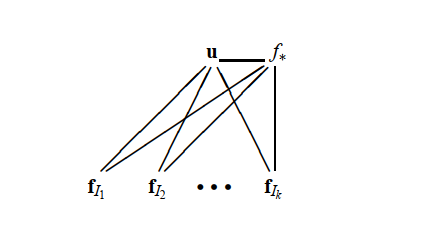
\includegraphics[width=0.5\textwidth]{image/transduction.png}
    \caption{Two views on Augmentation. One view is to see that the test latent function value $f_*$
is now part of the inducing variables u and therefore has access to the training latent
function values. An equivalent view is to consider that we have dropped the assumption
of conditional independence between $f_*$ and the training latent function values. Even if
$f_*$ has now direct access to each of the training fi, these still need to go through u to
talk to each other if they fall in conditionally independent blocks. We have in this figure
decided to recycle the graph for PITC from Figure 3 to show that all approximations we
have presented can be augmented, irrespective of what the approximation for the training
conditional is.} \label{fig:transduction}
\end{figure}

We can augment $u$ with $f_*$ as shown in the figure \ref{fig:transduction}, then the covariance of the conditional of $f_*$ is 0.
For example in SoR, if the test input is far from the training points, the mean will go to zero, but covariance will be small too, which is not 
what we expected. With the augment of the test point, by ensuring that there is always a basis function centered on the test case, there is a particularly big difference.
Although augmentation was initially proposed for a narrow set of circumstances, it is easily
applied to any of the approximations discussed.

But we should remember that

\begin{remark}
    A full non-degenerate Gaussian process cannot be augmented, a GP with a covariance function that has a
feature-space which is infinite dimensional, i.e. with basis functions everywhere.
\end{remark}

Let us compute the effective prior for the augmented SoR
\begin{equation}
    q_{\mathrm{ASoR}}(\mathbf{f}_{*},\mathbf{f})=\int q_{\mathrm{SoR}}(\mathbf{f}|f_{*},\mathbf{u})p(f_{*},\mathbf{u})d\mathbf{u}
\end{equation}
It is interesting to notice that this is also the effective prior that would result from augmenting the
DTC approximation, since $q_{\mathrm{SoR}}(\mathbf{f}|f_{*},\mathbf{u}) = q_{\mathrm{DTC}}(\mathbf{f}|f_{*},\mathbf{u})$.

\begin{remark}
    Augmented SoR (ASoR) is equivalent to augmented DTC (ADTC).
\end{remark}

Augmented DTC only differs from DTC in the additional presence of $f_*$ among the inducing variables in the training conditional. We can only expect 
augmented DTC to be a more accurate approximation than DTC, since adding an additional inducing variable can only help capture information
from $\bf y$. Therefore

\begin{remark}
    DTC is a less accurate (but cheaper) approximation than augmented SoR
\end{remark}

\subsection{On the Choice of the Inducing Variables}
We can use maximize the marginal
likelihood (also called the evidence) with respect to $X_u$ to get the inducing inputs.
\begin{equation}
    q({\bf y}|X_{\mathbf{u}})
    =\int \int p({\bf y}|{\bf f})q({\bf f}|{\bf u})p({\bf u}|X_{\mathbf{u}}) d{\bf u}\mathbf{d}{\bf f}=\int p({\bf y}|{\bf f})q({\bf f}|X_{\mathbf{u}})d{\bf f},
\end{equation}
which of course is independent of the test conditional. 

\begin{equation}
    \log q(\mathbf{y}|X_{\mathbf{u}})
    =-{\frac{1}{2}}\mathrm{log}|Q_{\mathbf{f,f}}+\Lambda|
    -{\textstyle\frac{1}{2}}\mathbf{y}^{\mathsf{T}}{\big(}Q_{\mathbf{f,f}}+\Lambda\big)^{-1}\mathbf{y}-{\textstyle\frac{n}{2}}\mathrm{log}(2\pi)
\end{equation}

\subsection{Other Methods and Conclusion}

\begin{figure}[htbp]
    \centering
    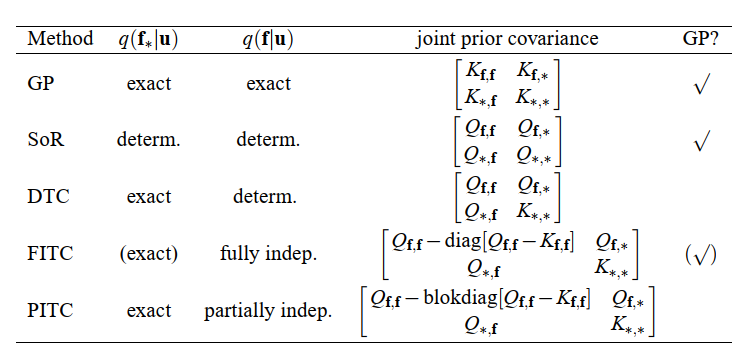
\includegraphics[width=0.8\textwidth]{image/sparse_gp_summary.png}
    \caption{summary of sparse GP} \label{fig:sparse_gp_summary}
\end{figure}

First is \mydefination{Nystrom Approximation}

\begin{equation}
    q(\mathbf f, \mathbf f f_*) = \mathcal N \left ( 0, \begin{bmatrix}
        Q_{\mathbf f, \mathbf f} & K_{\mathbf f, *} \\
        L_{*, \mathbf f} & K_{*, *}
    \end{bmatrix} \right )
\end{equation}

\begin{remark}
    The Nystrom Approximation does not correspond to a well-formed probabilistic model.
\end{remark}

The predictive distribution is 
\begin{equation}
    p(f_* | \mathbf y) = \mathcal N \left ( 
        K_{*, \mathbf f} [Q_{\mathbf f, \mathbf f} + \sigma^2 I]^{-1} \mathbf y, K_{*,  *} - K_{*, \mathbf f} [Q_{\mathbf f, \mathbf f} + \sigma^2 I]^{-1} k_{\mathbf f, *}    
    \right )
\end{equation}

Second one is \mydefination{Releavance Vector Machine}, which is given by
\begin{equation}
    f_* = \phi_* \mathbf w, \quad p(\mathbf w | A) = \mathcal N(0, A)
\end{equation}
where $\phi_* = [\phi_1(\mathbf x), \phi_2(\mathbf x), \ldots, \phi_m(\mathbf x)]$ is the (row) vector of responses of the $m$ basis functions, and
$A = \text{diag}(\alpha_1, \ldots, \alpha_m)$ is the diagonal matrix of joint prior precisions (inverse variances) of the weights.

\begin{remark}
    The RVM is equivalent to a degenerate Gaussian process with covariance function $k_{\mathrm{{RVM}}}(\mathbf{x}_{i},\mathbf{x}_{j})=\phi_{i}A^{-1}\phi_{j}^{\mathsf{T}}=\Sigma_{k=1}^{m}\alpha_{k}^{-1}\phi_{k}(\mathbf{x}_{i}) \phi_{k}(\mathbf{x}_{j})$
\end{remark}

\end{document}